\documentclass{tudelft-report}
%hier komen je packages wanneer nodig
\usepackage{minted, siunitx}
\usepackage{blindtext}
\usepackage{listings}
\usepackage{wrapfig}
\usepackage{float}
\usepackage{subcaption}
\usepackage{enumitem}
\usepackage{color} %red, green, blue, yellow, cyan, magenta, black, white
\renewcommand{\thesection}{\arabic{section}} %zodat die 0'etjes weg gaan :D
\makeatletter
% \textsubscript defined equivalent to \textsuperscript in latex.ltx
\DeclareRobustCommand*\textsubscript[1]{%
  \@textsubscript{\selectfont#1}}
\def\@textsubscript#1{%
  {\m@th\ensuremath{_{\mbox{\fontsize\sf@size\z@#1}}}}}
\makeatother
%voor subscript in titel, https://tex.stackexchange.com/questions/70981/sub-superscripts-in-headings-normal-text
\begin{document}

\frontmatter
\title[tudelft-white]{Design specification report}
\subtitle[tudelft-black]{EPO-3} 
\author[tudelft-white]{A5}       % hier kan je je groepsnummer invoeren
\setlength{\parindent}{0ex}
\setlength{\parskip}{0.7em}


\covertext[tudelft-white]{
    {\color{black} \today}
    \vspace{300pt} % dit een beetje aanpassen om het mooi te maken
    \begin{flushright}
        Joris van Breukelen ~~~\textit{4704967}\\
        Ferdi Dabak, ~~~\textit{4674332}\\
        Hitesh Dialani,      ~~~\textit{4748153}\\
        Talha Kuruoglu, ~~~\textit{4718569}\\ 
        Michael Miao, ~~~\textit{4684206}\\
        Daniel van Paassen,         ~~~\textit{4724968} \\
        Koen van Remundt,      ~~~\textit{4601793}\\
        Tim van der Spijk, ~~~\textit{4693817}\\
        Daniel Vlaardingerbroek, ~~~\textit{4580834}\\
        
                   
    \end{flushright}
}
\makecover[split]

\thispagestyle{empty}
\vspace{30mm}
%\begin{center}
%    \Large \bf Abstract
%\end{center}
%An abstract is a brief summary of a research article, thesis, review, conference proceeding, or any in-depth analysis of a particular subject and is often used to help the reader quickly ascertain the paper's purpose.

\tableofcontents

\mainmatter
\section{Introduction}
Bomberman is a game originally created and published by Hudson Soft inc. in the United Kingdom in the year 1983. At this first introduction the game was called "Eric and the Floaters". The game was re-released later as "Bomberman" . The game became a huge hit and was recreated numerous of times by several different companies including Hudson Soft inc. \cite{mobygames}.\\

The goal of the game is to 'kill' the opponent by hitting them with an exploding bomb. Different versions of the game made it more difficult to reach the opponent by using for example crates that block the player from walking. This increases the time before players can start attacking each other.\\

All team members of the A5 group played this game as a kid. This created a mutual interest to create this game using only hardware. This will be done by first creating the game in VHDL. After that the VHDL will be synthesized and tested on an FPGA. If everything is working properly, the game will be created on a wafer which uses 180nm technology. \\%is this true??

In this report, a brief outline of the design process will be discussed.\\

%\begin{figure}[h]
 %   \centering
  %  
\includegraphics[width=40mm]{Figures/ericfloaters.jpg}
   % \caption{The front cover of the first bomberman game}
    %\label{fig:first}
%\end{figure}


\section{Global overview: Specification \& boundaries of the system}
\begin{figure}[H]
\begin{subfigure}{.5\textwidth}
    \centering
    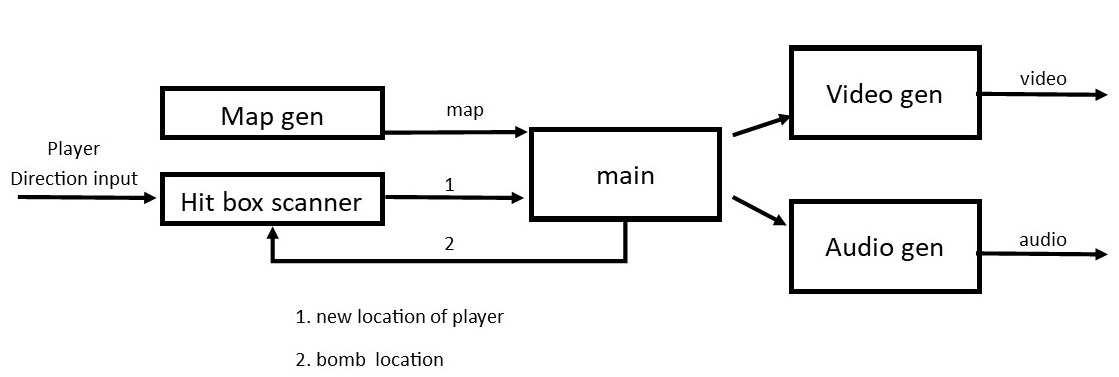
\includegraphics[width=1\linewidth]{Figures/function_block_diagram.jpg}
    \caption{The functional block diagram of the sub-blocks of the bomberman game with inputs, outputs and internal signals defined by arrows.}
    \label{fig:blockdiagram}
    \end{subfigure}% 
    \begin{subfigure}{.5\textwidth}
    \centering
    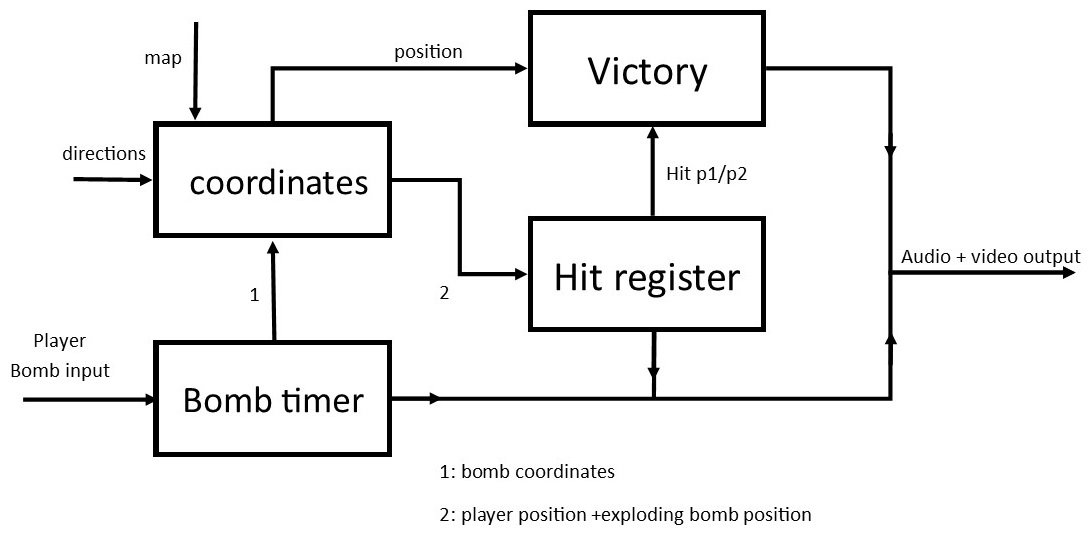
\includegraphics[width=1\linewidth]{Figures/main_block.jpg}
    \caption{The expanded functional block diagram of the main module from Fig. \ref{fig:blockdiagram} with input and outputs defined by arrows.}
    \label{fig:mainblockdiagram}
\end{subfigure}
\end{figure}

The goal is to create a 2-player multiplayer bomberman game. Each player has to be able to move in 4 directions and place bombs. For this, 5 inputs are needed per player. Adding the clock and reset input, a total of 12 inputs is needed. With 16 inputs available, this is not a problem. The reset input will put all Finite State Machines (in short: FSM's) in the reset state and can be used when a game is finished to restart the game. To visually interface with the user, an image is projected on a display through VGA. Optionally sound effects and a victory screen can be added. VGA requires 5 pins to work properly, this is not a problem with the total of 16 output pins. The audio should also be perfectly possible to implement with the amount of output pins that are available.\\

The maximum clock frequency of the chip is 12.5 MHz, which is not sufficient for the pixel-frequency of the VGA. This requires a clock frequency of 25 MHz. This will be resolved by reducing the resolution of the output. The resolution can be reduced, seen as the image quality of our game is not the focus of the project.\\

The FSM's must be a Moore machines. This means that the output of each FSM can only depend on the state of the machine, not on the input of the machine. The FSM's work at the rising clock edge, so all subsystems will be synchronized. \\

The size of the chip technology limits the amount of flipflops that can be used in the design. The maximum would be around 600 flipflops. This means that everything concerning signals and variables must be as efficient as possible in order to waste as few flipflops as possible. This is very crucial in a lot of modules, for example the coordinates of grid.

The general idea of the system is that the input of movement of the players should be checked by the \textbf{hitbox} module in Fig. \ref{fig:blockdiagram}. If it is possible to move, the \textbf{hitbox} passes the new coordinates to the \textbf{main} module. This module consists of the \textbf{coordinates}, \textbf{bomb timer}, \textbf{victory} and \textbf{Hit register} sub-modules, these are further explained in Section \ref{overview}. 
\section{Overview per block}
\label{overview}

\subsection{Map generation}\label{Map generation}
The game will be played on a map that consists of a 9 by 9 grid that is surrounded by walls, resulting in a 11 x 11 field. There are also 16 walls within the playing field, which do not change during the course of the game. This results in a total of 65 playable spaces on which players walk and destructible crates or blocks can be placed, as shown in Fig. \ref{fig:layout}. The location of the crates is predetermined, but can be programmed to be randomized if time allows. At the start of the game players 1 and 2 are placed in the top left and bottom right corner respectively. The data of the grid is used as input in the block: Coordinates in section \ref{Coordinates}. This way every tile has a binary value for whether or not there is a crate present, based on this the right output can be determined in the coordinates block. The map generation is where this layout is defined.

\begin{figure}[H]
    \centering
    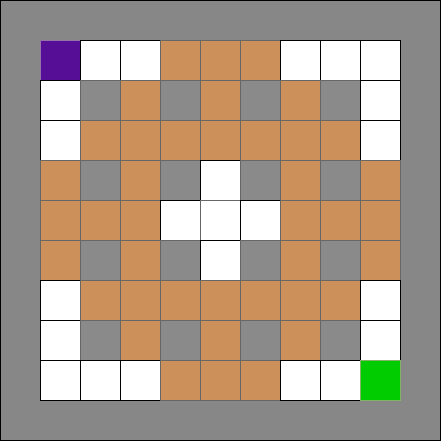
\includegraphics[width=0.4\textwidth]{Figures/bomberman.png}
    \caption{The layout of the bomberman grid, in which grey stands for walls, brown for crates, white the empty tiles and the remaining colours for the players.}
    \label{fig:layout}
\end{figure}


\subsection{Hitbox scanner}\label{Hitbox Scanner}
Another part of the design is how the player is able to move. The movement is based on the current position of the player and the inputs that are given. The players' locations are stored in two dimensional coordinates. The players are not allowed to walk towards spaces that contain either walls, crates or bombs. When the player places a bomb, it appears at the spot the player is currently at. The player should be able to move away from this spot. Furthermore, the player should be limited on how fast they can give inputs. Therefore a system has to be developed that makes sure the system waits for a certain duration before it becomes sensitive for the user's inputs again. This makes sure both players have the ability to move at the same speed. 

\subsection{Coordinates}\label{Coordinates}
The Coordinates block will send bomb location and players locations as output to the Hit Register and the Victory block. The generated map (\ref{Map generation} and the bomb timing signals \ref{BombTimer} are essential inputs of the Coordinates entity. Moreover, the player coordinates and bomb location are  important input.

Three distinct components are present at the output of the Coordinates block. Firstly, a propagated map. This map is merely subject to graphical changes, it forms the fundamental graphic layer presented on the screen. Another output makes sure the bombs are visible at the correct tiles at the appropriate times, overlapping the map. To achieve this, player positions and bomb timing signals will be used. Lastly, the player positions will be propagated.


%As for the inputs of Coordinates: Firstly the map generator will send the default layout shown in Fig. \ref{fig:layout}, from which the tile type and tile location together with both players starting points will be stored. After which the desired location for the movement and/or bomb placement from both players will be taken as input. Lastly, the Bomb Timer is the final input. The coordinates of the detonated bombs are important for the win condition.
 
 The coordinates of the bombs will be implemented using two 4-bit coordinates (\texttt{x} and \texttt{y}), the same goes for the player positions. This method is beneficial, because these elements are relatively scarce.
 %and active throughout gameplay (bombs explode with a certain tile radius, players move from tile to tile). The \texttt{x} and \texttt{y} values can be used efficiently to model these actions in VHDL.
 For the crates: each tile is represented by a flip flop, which can either contain a logic \texttt{'1'} (crate present on tile) or \texttt{'0'} (crate absent on tile). The walls will be hard coded as a logic \texttt{'1'} (wall present on tile) or \texttt{'0'} (wall absent on tile).
 
 \subsection{Bomb Timer}\label{BombTimer}
 Every bomb on the field needs their own timer. This timer is there to give the player time to move away from the bomb when it gets placed. Because timers usually require a large amount of flip-flops, some precautionary measures have to be taken: The timers will use the clock signal that will get generated for the VGA output, this will significantly reduce the amount of flip-flops necessary, these timers will also get reused by the Hit Register. When a bomb has been placed, the first timer of the Bomb timer will then start running. If another bomb gets placed, the Bomb timer will recognize that the first timer is in use and switch to the second timer. This will ensure that all bomb timers will run independently from each other.
 
 \subsection{Hit Register}
 When a bomb detonates, the bomb has a sort of radius in which it is checked if a player (or box in later iterations) is present. This is not a round like radius, but a horizontal and vertical line, in which everybody who is present (even the player who placed the bomb) loses the game or a life in later iterations. The first thing that is checked, is whether the exploding bomb has any hard walls next to it. %In the case that there is no wall present right next to the bomb, there will be no wall further than that unless it is the wall which blocks off the edge of the map. This needs to be done only once. If there is a wall above the bomb, than there must be a wall below the bomb. This is also the case with left and right. After that, 2 tiles on each side of the bomb will be checked on players or destructible crates.
 Then it will check if there are any players or crates inside the radius without going through a wall, meaning that the explosion cannot go through walls. A crate will be destroyed if it is detected. If a player gets detected, a signal will be sent to the Victory block.

\subsection{Victory}
This block can be seen as a multiplexer, where in a normal situation (nobody got hit) the output of coordinates is passed on to the output block and Hitbox scanner. In the case that somebody does get hit by a bomb, a victory screen will be passed on to the output. 
 
 \subsection{Output}\label{Output}
 To actually play the game it has to be displayed on a monitor. This will be done by using the VGA protocol. Although a VGA connector consists of 15 pins, only 5 of these will be used for the game. Three pins are needed to determine the colour of a specific pixel which is determined by the other two pins. Each of the three pins for the colour corresponds to a different colour, so for the colours red, green and blue. Each one can be set to off or on. Combinations of red, green and blue can make other colours. Therefore in total $2^3 = 8$ colours can be generated. Each pixel on the screen has to be coloured separately, this happens on the rising clock edge. The screen consists of 640x480 pixels. The refresh rate should be 60 Hz. There is also some time required to change from row and to start a new frame (with the two other pins). So in total a clock frequency of 25.175 MHz is required. Since the clock frequency of the chip is just 12.5 MHz, the resolution will be lower. This is in the case of this game not a very big issue. 
 The output module receives all the information of the coordinates from the coordinates module. This module should use this information to display the players, bombs, crates and the entire grid on the right pixel locations. Also sound effects can be added later on when for example a bomb detonates. 
\section{House Rules}
To ensure that everybody is on the same page regarding for example the topics of meeting times and penalties, a set of house rules have been made. Everybody in this project group have thought about them and agreed to them. These house rules can be found below.

\begin{itemize}[noitemsep]
    \item The group members all come together on Mondays and Thursday from 8:45 till 12:30.
    \item There will be two meeting on those days, one at the start and one at the end of the session.
    \item If somebody is more than 5 minutes late without a good reason they will have to bring food for the whole group, this will be done at the next meeting.
    \item Every morning a break of 15 minutes is allowed.
    \item 24 hours before a deadline everything has to be finished, so team members have time to review it. 
    \item During meetings one person talks at a time.
\end{itemize}

\subsection{Planning}
A good time plan and division of the subsystems is very important, this is to make sure that the workload of this project is spread evenly in between the students and that there will be enough time to finish this project. The project has been divided into four modules, these modules can be found in Table \ref{tab:mod_div}.

The schedule that was shown in a presentation at the beginning of this project will be used as time plan \cite{Presentation}. As a group it has been decided that additional days might be necessary to ensure that the project can be finished with the best result possible, so additional meetings will be planned if it is deemed necessary.

\begin{table}[ht!]
    \centering
    \caption{Table with the module divisions.}
    \begin{tabular}{|l|r|}
    \hline
    Module                              & Students \\
    \hline
    Map generator \& Hitbox scanner     &  Michael, Talha and Daniel P.\\
    Coördinates                         & Ferdi and Hitesh\\
    Output (VGA + sound)                & Joris and Tim\\
    Bomb timer, Hit Register \& Victory & Koen and Daniel V.\\
     \hline
    \end{tabular}
    
    \label{tab:mod_div}
\end{table}
\section{Mutual Tuning}
\subsection{Map Generator}
The Map Generator block can be seen in Fig. \ref{fig:blockdiagram}. The outputs of the Map Generator consists of the crates and the walls both send by a 121 bit-vector to the block "main". So the block main gets the initial game map. 

\subsection{Hitbox scanner}
The hitbox scanner can be seen in Fig. \ref{fig:blockdiagram}. The input signals that consist of the directional movement of the players comes from the joystick.The hit box scanner has a clock signal of 12.5 MHz and a reset as input. The new player coordinates will be sent to the main module in a 8 bit-vector per player.The speed of the players will be adjusted with a "cooldown" state, by making a counter that counts until 0.25 seconds.  

\subsection{Main}
The main block is zoomed in at Fig. \ref{fig:mainblockdiagram}. The function of the coordinates block is described at Section \ref{Coordinates}. The input from the map generator is the initial map. The coordinates block will also have an input signal of two 4-bit vectors for the bombs, coming from the bomb timer. The coordinates block will send an output to the hitbox scanner with an updated map containing the new player coordinates, bomb(4 bit-vector) location and crate(121 bit-vector) location.
\\
\\
\noindent
The Bomb timer gets a 2-bit vector input from the buttons that are pressed by each player to drop a bomb in the game, one bit to determine if a bomb is placed and 1 bit to determine which player dropped the bomb. The bomb timer will use the same clock signal frequency that gets generated for the VGA output, which is 60 Hz. There will also be an output to the audio block. The coordinates will get a 4-bit x and y position vector with the bomb coordinates and signal that a bomb is placed. 
\\
\\
\noindent
The hit register has an input of a 28 bit-vector consisting of the bomb and player location from coordinates block. The hit register will send an output to block Victory if any player is hit by a bomb.In total there is an output of 7 bits per bomb. Hit register will also have an output to the video and possible audio generator.


\section{Testability}
\subsection{Controllability and Observability}
Controllability defines the difficulty or cost of setting a certain output or node to a value of choice (be it 1 or 0)\cite{CandO}. This controllability decreases when the system that is being tested becomes more complex. A single node has the highest controllability of 1. This is because the input and output are directly connected to each other and thus are the same. \\
Another value which is useful for testability is observability. Observability measures the cost of observing any value on a node\cite{CandO}. The observability, just like the controllability, decreases as the system that is being tested increases in complexity. Although there is a correlation between observability and controllability, they are not the same or inverses of each other.

\subsection{Black-box and white-box testing}
Black-box and white-box testing are two very important forms of testing which are still useful to know the difference of. Black-box testing is testing without looking at what is happening between components or parts of the design. This way of testing is a good way if it is thought that the system is functional in the way it is intended to be. \cite{informationvisualization}. If this is not the case, it may become evident what error is by looking at the type of output error the system is producing. If this also fails,  it is advisable to resort to white-box tests.\\
White-box or clear-box testing is testing parts of your design individually. This helps to easily see where the error in the system is. By separating parts of the system into subsystems,  it is advisable to resort to white-box tests and thus increase the controllability and observability. 
Black-box and white-box testing are meant to be used together\cite{informationvisualization}. Black-box testing is easier and less time consuming than white-box testing, but white-box testing goes in much more depth than black-box testing and makes spotting the error easier. In the beginning of this project white-box testing will mostly be used since most subsystems still need to be built. When everybody has made their subsystem and all subsystems are combined to make the large system, black-box testing is possible and be used to check for errors often.
\section{Conclusion}
To sum up, the group is devoted to designing a working Bomberman game for the EPO-3 project. To achieve this goal, the group is divided into several smaller groups that work on a specific part of the game. The several individually designed entities, mentioned in the report, will ultimately be combined in a higher level entity that will be the final deliverable. Communication between these smaller groups is essential, because a lot of aspects of the initial design plan can still change due to unforeseen difficulties.

For now, every member of the group knows what needs to be done and tasks are divided clearly. The team seems to work well together, and in combination with the rules and agreements that have been set up a good fundamental working environment has been created. From this point forward, the group will work towards a finalized Bomberman game.

%\appendix
%\chapter{Images}

% en meer appendices...


\bibliography{report}

\end{document}